% !TEX root = ./correctness-deciders.tex
\title{Correctness of bbchallenge's deciders}
\author{
        Tristan St\'{e}rin, Alexandre Jouandin and Sébastien Ohleyer
}

\documentclass[a4paper,british]{article}
\usepackage{babel}
\usepackage[utf8]{inputenc}
\usepackage[margin=1in]{geometry}
%\usepackage{subfig}
\usepackage[hidelinks]{hyperref}
\usepackage{caption}
\usepackage{subcaption}
\usepackage{tikz}

\usepackage{algorithm}
\usepackage[noend]{algpseudocode}

\usepackage{graphicx}

\usepackage{amsmath,amsfonts,amssymb,amsthm}


\newtheorem{theorem}{Theorem}
\newtheorem{definition}[theorem]{Definition}
\newtheorem{lemma}[theorem]{Lemma}
\newtheorem{proposition}[theorem]{Proposition}
\newtheorem{corollary}[theorem]{Corollary}

\newtheorem{observation}[theorem]{Observation}
\newtheorem{example}[theorem]{Example}
\newtheorem{remark}[theorem]{Remark}


\usepackage{microtype,xspace,wrapfig,multicol} 
\usepackage[textsize=tiny,color=lightgray]{todonotes} 
\usepackage[normalem]{ulem} % sout

\newcommand{\ts}[1]{{\color{red}#1}}
\newcommand{\tsi}[1]{\todo[inline]{TS: #1}}
\newcommand{\tsm}[1]{\todo{TS: #1}}
\newcommand{\tss}[2]{{\ts{\sout{#1}}} {\ts{#2}}}
\newcommand{\tabi}{\hspace{\algorithmicindent}}

\usepackage{xcolor}

\definecolor{colorA}{RGB}{255,0,0}
\definecolor{colorB}{RGB}{255,128,0}
\definecolor{colorC}{RGB}{0,0,255}
\definecolor{colorD}{RGB}{0,255,0}
\definecolor{colorE}{RGB}{255,0,255}

\begin{document}
\date{}
\maketitle

\begin{abstract}
        The Busy Beaver Challenge (or bbchallenge) aims at collaboratively solving the following conjecture: ``BB(5) = 47,176,870'' [Aaronson, 2020]\nocite{BusyBeaverFrontier}. This goal amounts to decide whether or not 88,664,064 Turing machines with 5-state halt or not -- starting from all-0 tape. In order to decide the behavior of these machines we write \textit{deciders}. A decider is a program that takes as input a Turing machine and outputs \texttt{true} if it is able to tell whether the machine halts or not. Each decider is specialised in recognising a particular type of behavior that can be decided. 
        
        In this document we are concerned with proving the correctness of these deciders programs. More context and information about this methodology are available at \url{https://bbchallenge.org}.
\end{abstract}
\tableofcontents

\section{Conventions}

\begin{table}[h!]
  \centering
  \begin{tabular}{lll}
    & 0   & 1   \\
  A & 1RB & 1LC \\
  B & 1RC & 1RB \\
  C & 1RD & 0LE \\
  D & 1LA & 1LD \\
  E & - - - & 0LE
  \end{tabular}
  \caption{Transition table of the current 5-state busy beaver champion: it halts after 47,176,870 steps.\\\url{https://bbchallenge.org/1RB1LC1RC1RB1RD0LE1LA1LD---0LA&status=halt}}
  \end{table}\label{table:bb5}

The set $\mathbb{N}$ denotes $\{0,1,2\dots\}$. 

\paragraph*{Turing machines.}The Turing machines that are studied in the context of bbchallenge use a binary alphabet and a single bi-infinite tape. Machine transitions are either undefined (in which case the machine halts) or given by (a) a symbol to write (b) a direction to move (right or left) and (c) a state to go to. Table~\ref{table:bb5} gives the transition table of the current 5-state busy beaver champion. The machine halts after 47,176,870 steps (starting from all-0 tape) when it reads a 0 in state E, which is undefined.

A \textit{configuration} of a Turing machine is defined by the 3-tuple: (i) state (ii) position of the head (iii) content of the memory tape. In the context of bbchallenge, \textit{the initial configuration} of a machine is always (i) state is 0, i.e. the first state to appear in the machine's description (ii) head's position is 0 (iii) the initial tape is all-0 -- i.e. each memory cell is containing 0. We write $c_1 \vdash_\mathcal{M} c_2$ if a configuration $c_2$ is obtained from $c_1$ in one computation step of machine $\mathcal{M}$. We omit $\mathcal{M}$ if it is clear from context. We let $c_1 \vdash^s c_2$ denote a sequence of $s$ computation steps, and let  $c_1 \vdash^* c_2$ denote zero or more computation steps. % exact same wording as in https://dna.hamilton.ie/assets/dw/NearyWoodsFCT09.pdf
We write $c_1 \vdash \bot$ if the machine halts after executing one computation step from configuration $c_1$. In the context of bbchallenge, halting happens when an undefined machine transition  is met i.e. no instruction is given for when the machine is in the state, tape position and tape corresponding to configuration $c_1$.

\paragraph*{Space-time diagram.} We use space-time diagrams to give a visual representation of the behavior of a given machine. The space-time diagram of machine $\mathcal{M}$ is an image where the $i^\text{th}$ row of the image gives:
\begin{enumerate}
  \item The content of the tape after $i$ steps (black is 0 and white is 1).
  \item The position of the head is colored to give state information using the following colours for 5-state machines: \textcolor{colorA}{A},  \textcolor{colorB}{B},  \textcolor{colorC}{C},  \textcolor{colorD}{D},  \textcolor{colorE}{E}.
\end{enumerate}

\section{Decider for ``Cyclers''}\label{sec:cyclers}

\begin{figure}[h!]
\centering

\includegraphics[width=0.4\textwidth]{space-time-diagrams/cycler_279081.pdf}
\hspace{2ex}
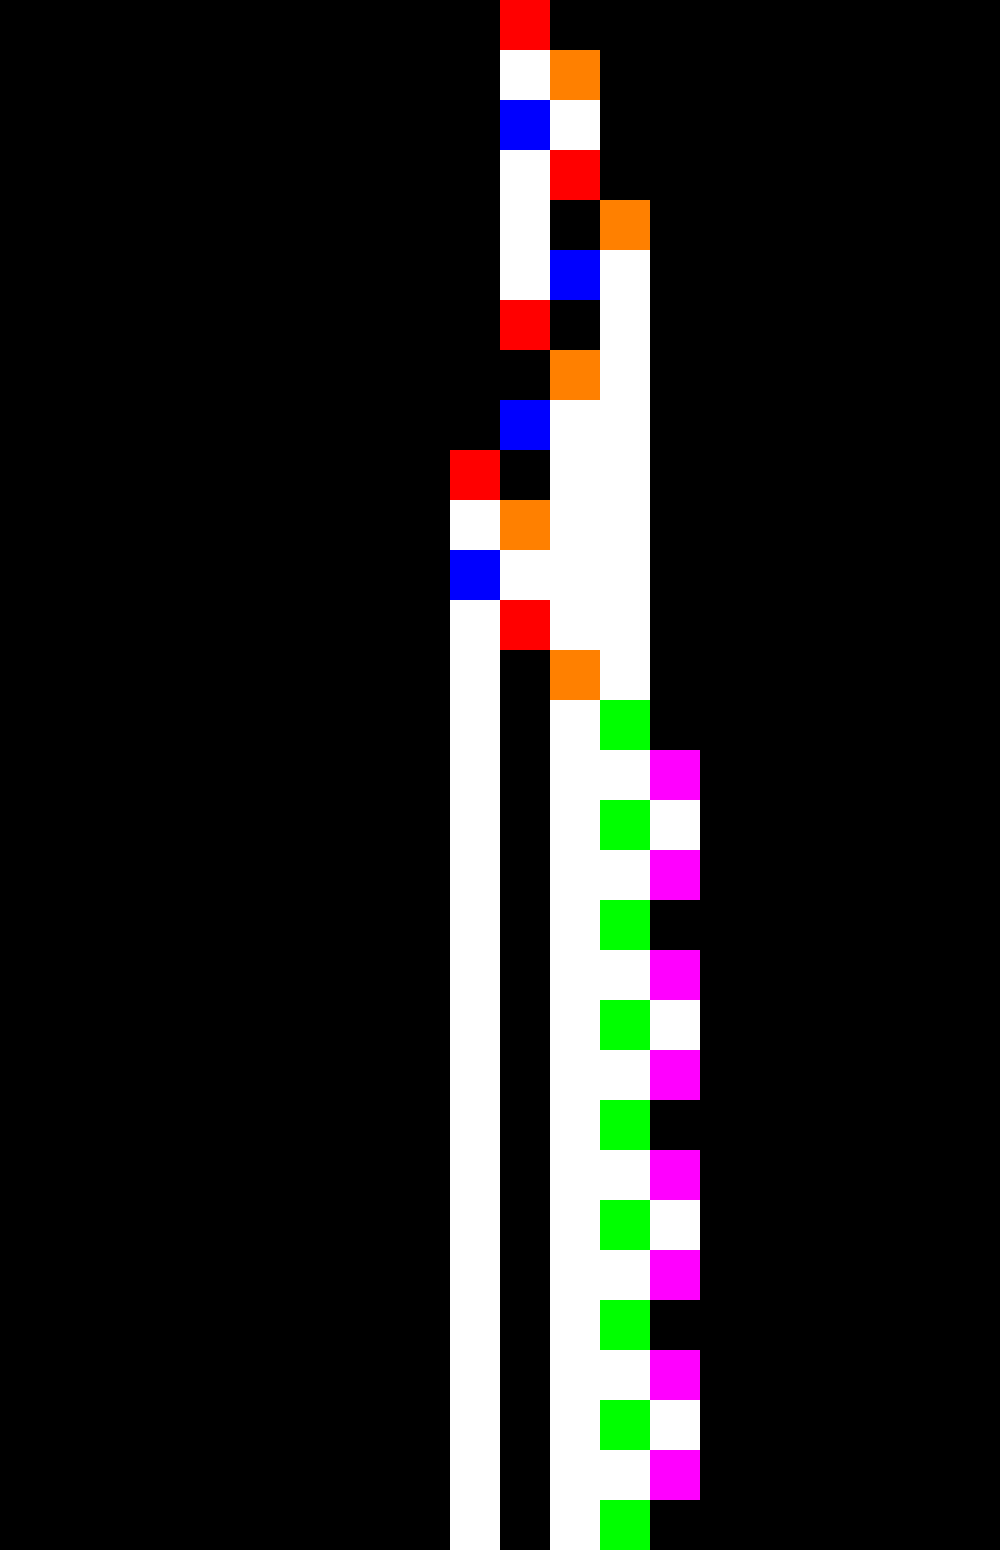
\includegraphics[width=0.4\textwidth]{space-time-diagrams/cycler_4239083.pdf}
\caption{Space-time diagrams of the 30 first steps of bbchallenge's machines \#279,081 (left) and \#4,239,083 (right) which are both ``Cyclers'': they eventually repeat the same configuration for ever. \\
Access the machines at \url{https://bbchallenge/279081} and 
\url{https://bbchallenge/4239083}.}\label{fig:cyclers}
\end{figure}

The goal of this decider is to recognise Turing machines that cycle through the same configurations for ever. Such machines never halt. The method is simple: remember every configuration seen by a machine and return \texttt{true} if one is visited twice. A time limit (maximum number of steps) is also given for running the test in practice: the algorithm recognises any machine whose cycle fits within this limit\footnote{In practice, for machines with 5 states the decider was run with 1000 steps time limit.}.


\begin{example}\normalfont
Figure~\ref{fig:cyclers} gives the space-time diagrams of the 30 first iterations of two ``Cyclers'' machines: bbchallenge's machines \#279,081 (left) and \#4,239,083 (right). Refer to \url{https://bbchallenge/279081} and 
\url{https://bbchallenge/4239083} for their transition tables. From these space-time diagrams we see that the machines eventually repeat the same configuration.
\end{example}

\newpage
\subsection{Pseudocode}

We assume that we are given a Turing Machine type \textbf{TM} that encodes the transition table of a machine as well as a procedure \textbf{TuringMachineStep}(machine,configuration) which computes the next configuration of a Turing machine from the given configuration or \textbf{nil} if the machine halts at that step.

\begin{algorithm}
        \caption{{\sc decider-cylers}}\label{alg:cyclers}

        \begin{algorithmic}[1]

                \State \textbf{struct} Configuration \{
                \State \tabi\textbf{int} state
                \State \tabi\textbf{int} headPosition
                \State \tabi\textbf{int $\boldsymbol{\to}$ int} tape
                \State \}
                \State 
                \Procedure{\textbf{bool} {\sc decider-cylers}}{\textbf{TM} machine,\textbf{int} timeLimit}
                \State \textbf{Configuration} currConfiguration = \{.state = 0,$\,$.headPosition = 0,$\,$ .tape = \{0:0\}\}
                \State \textbf{Set$\boldsymbol{<}$Configuration$\boldsymbol{>}$} configurationsSeen = \{\}
                \State \textbf{int} currTime = 0

                \While{currTime $<$ timeLimit}
                \If{currConfiguration \textbf{in} configurationsSeen}
                \State \textbf{return} true
                \EndIf
                \State configurationsSeen.\textbf{insert}(currConfiguration)

                \State currConfiguration = \textbf{TuringMachineStep}(machine,currConfiguration)
                \State currTime += 1


                \If{currConfiguration == \textbf{nil}}
                \State \textbf{return} false //machine has halted, it is not a Cycler
                \EndIf
                \EndWhile

                \State \textbf{return} false
                \EndProcedure

        \end{algorithmic}
\end{algorithm}

\subsection{Correctness}



\begin{theorem}\label{th:cyclers}\normalfont Let $\mathcal{M}$ be a Turing machine and $t \in \mathbb{N}$ a time limit. Let $c_0$ be the initial configuration of the machine. There exists $i\in\mathbb{N}$ and $j\in\mathbb{N}$ such that $c_0 \vdash^i c_i \vdash^j c_i$ with $i+j \leq t$ if and only if {\sc decider-cyclers}($\mathcal{M}$,$t$) returns \texttt{true} (Algorithm~\ref{alg:cyclers}).
\end{theorem}
\begin{proof}
        This follows directly from the behavior of {\sc decider-cyclers}($\mathcal{M}$,$t$): all intermediate configurations below time $t$ are recorded and the algorithm returns \texttt{true} if and only if one is visited twice. This mathematically translates to
        there exists $i\in\mathbb{N}$ and $j\in\mathbb{N}$ such that $c_0 \vdash^i c_i \vdash^j c_i$ with $i+j \leq t$, which is what we want. Index $i$ corresponds to the first time that $c_i$ is seen (l.13 in Algorithm~\ref{alg:cyclers}) while index $j$ corresponds to the second time that $c_i$ is seen (l.11 in Algorithm~\ref{alg:cyclers}).
\end{proof}

\begin{corollary}\normalfont
        Let $\mathcal{M}$ be a Turing machine and $t \in \mathbb{N}$ a time limit. If {\sc decider-cyclers}($\mathcal{M}$,$t$) returns \texttt{true} then the behavior of $\mathcal{M}$ from all-0 tape has been decided: $\mathcal{M}$ does not halt.
\end{corollary}
\begin{proof}
        By Theorem~\ref{th:cyclers}, there exists $i\in\mathbb{N}$ and $j\in\mathbb{N}$ such that $c_0 \vdash^i c_i \vdash^j c_i$ with $i+j \leq t$. It follows that for all $k\in\mathbb{N}$, $c_0 \vdash^{i+kj} c_i$. The machine never halts as it will visit $c_i$ infinitely often.
\end{proof}

\subsection{Results}

The decider was coded in \texttt{golang} and is accessible at this link: \url{https://github.com/bbchallenge/bbchallenge-deciders/tree/main/decider-cyclers}.

The decider found 11,229,238 ``Cyclers'', out of 88,664,064 machines in the seed database of the Busy Beaver Challenge (c.f. \url{https://bbchallenge.org/method#seed-database}). More information about these results are available at: \url{https://discuss.bbchallenge.org/t/decider-cyclers/33}.

\newpage
\section{Decider for ``Translated cyclers''}\label{sec:translated-cyclers}

\begin{figure}[h!]
  \centering
  % 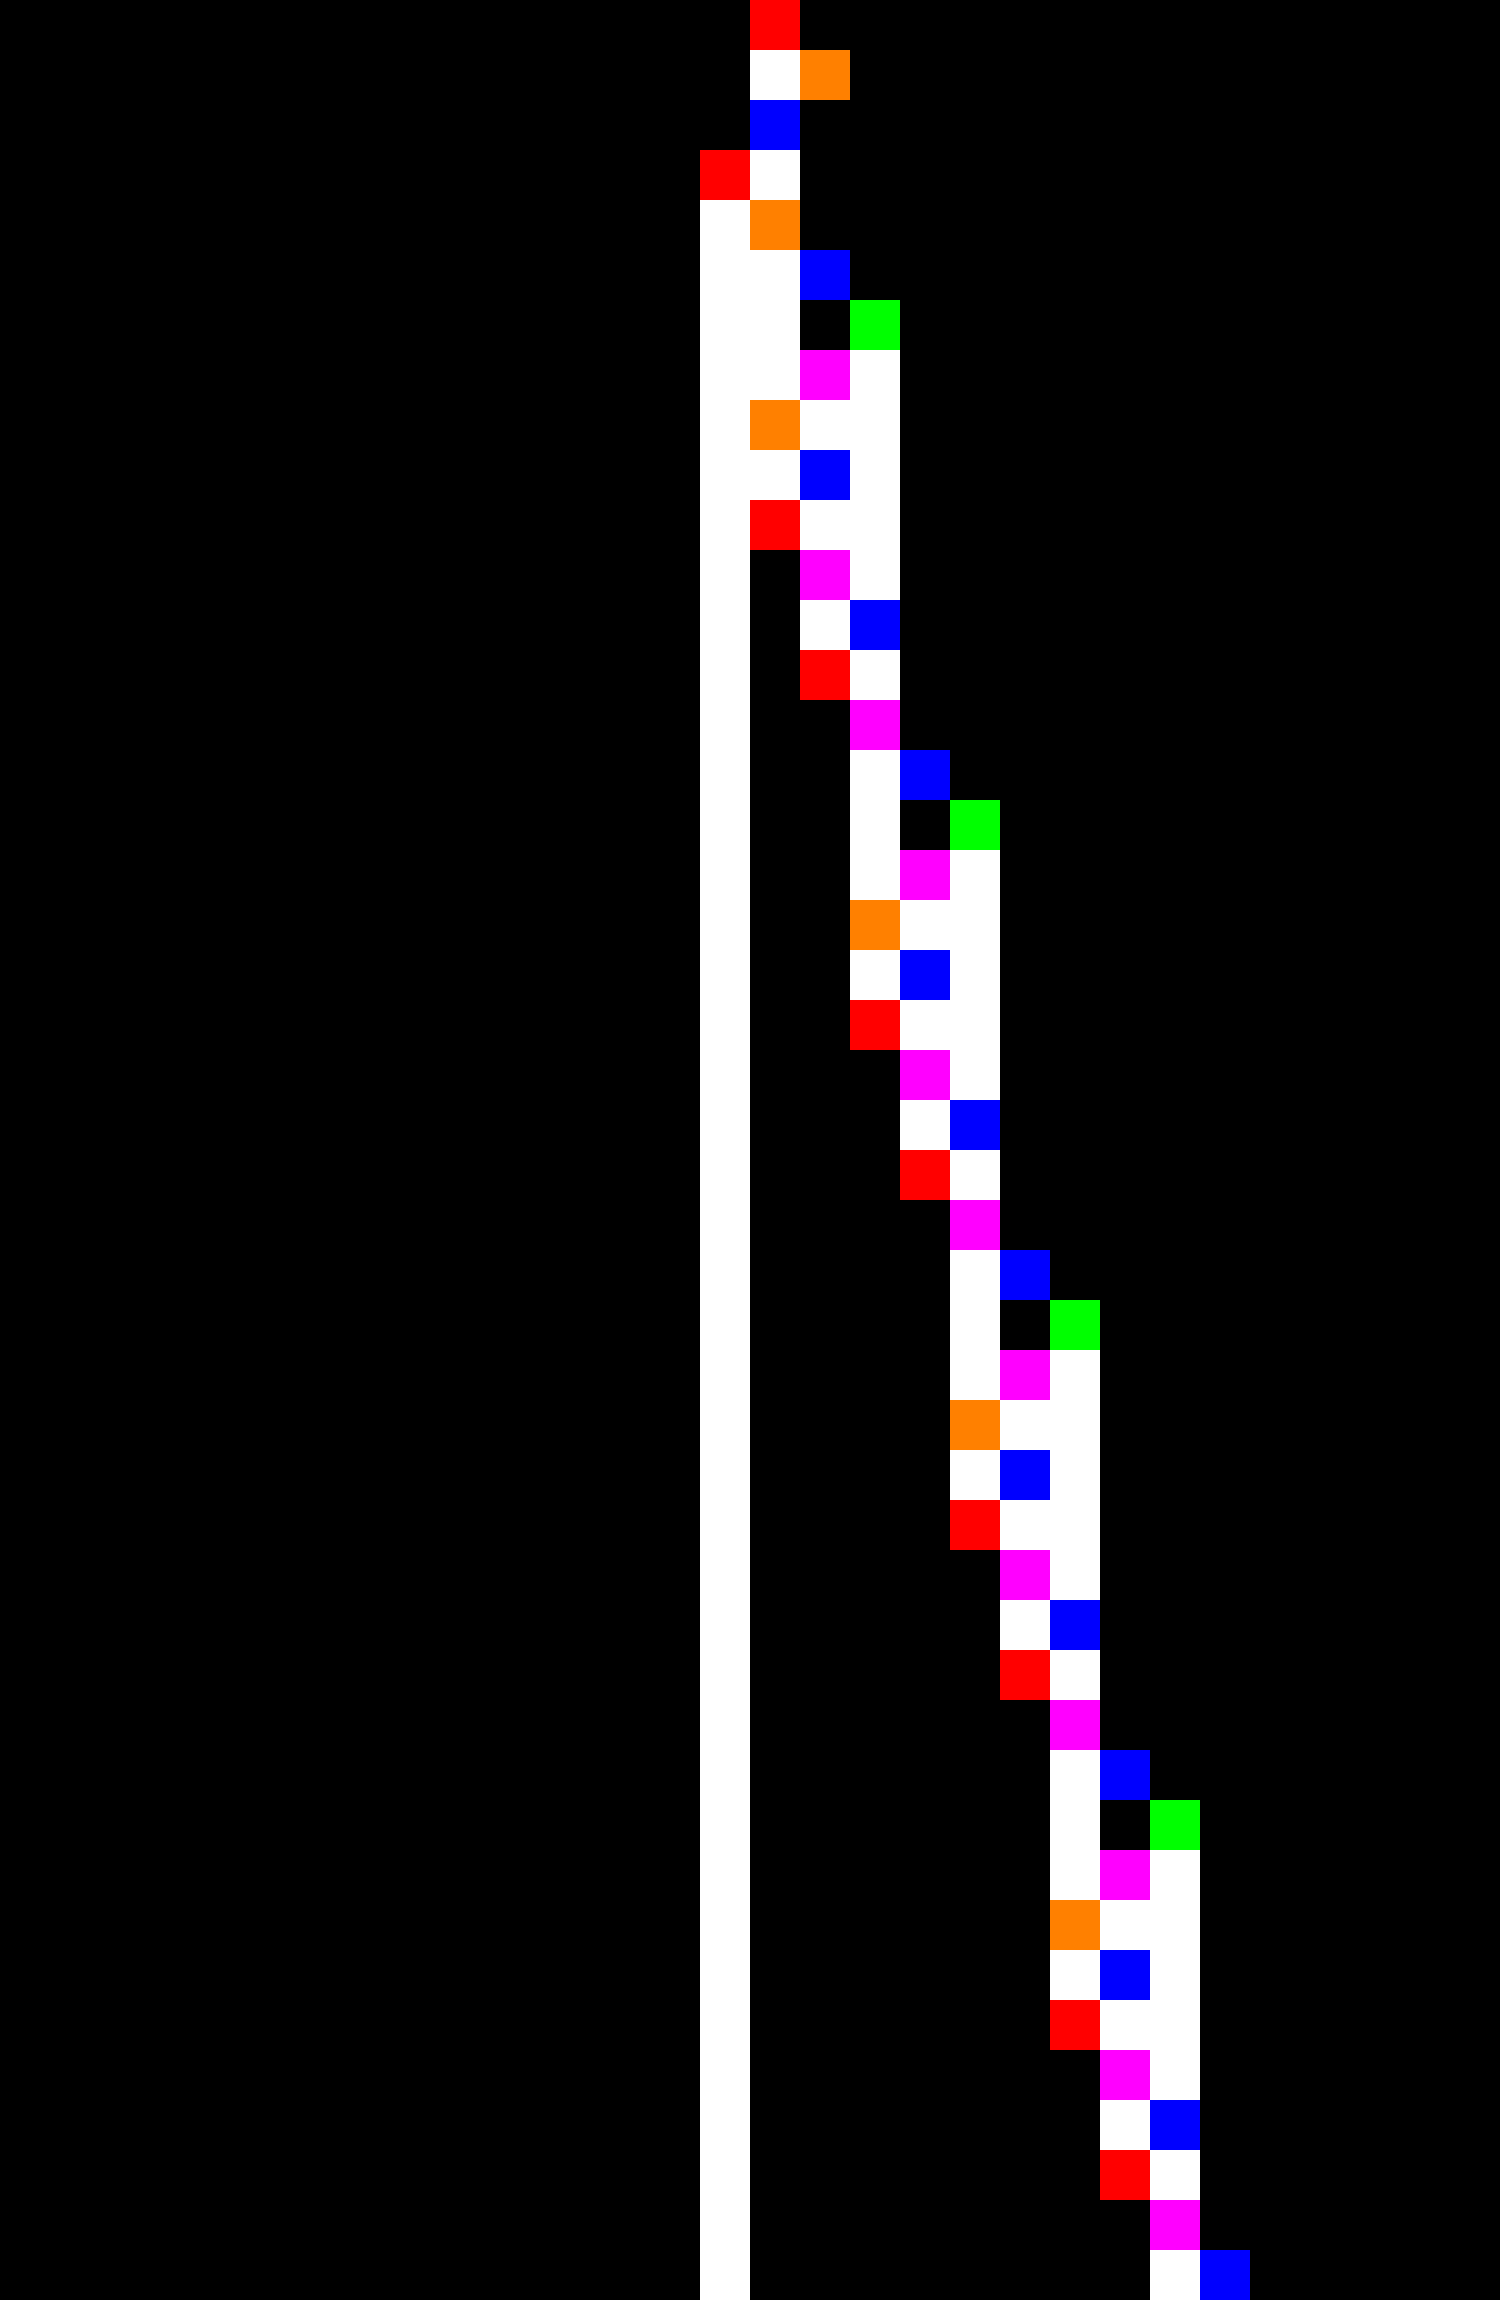
\includegraphics[width=0.5\textwidth]{space-time-diagrams/translated_cycler_44394115.pdf}
  % \hspace{2ex}
  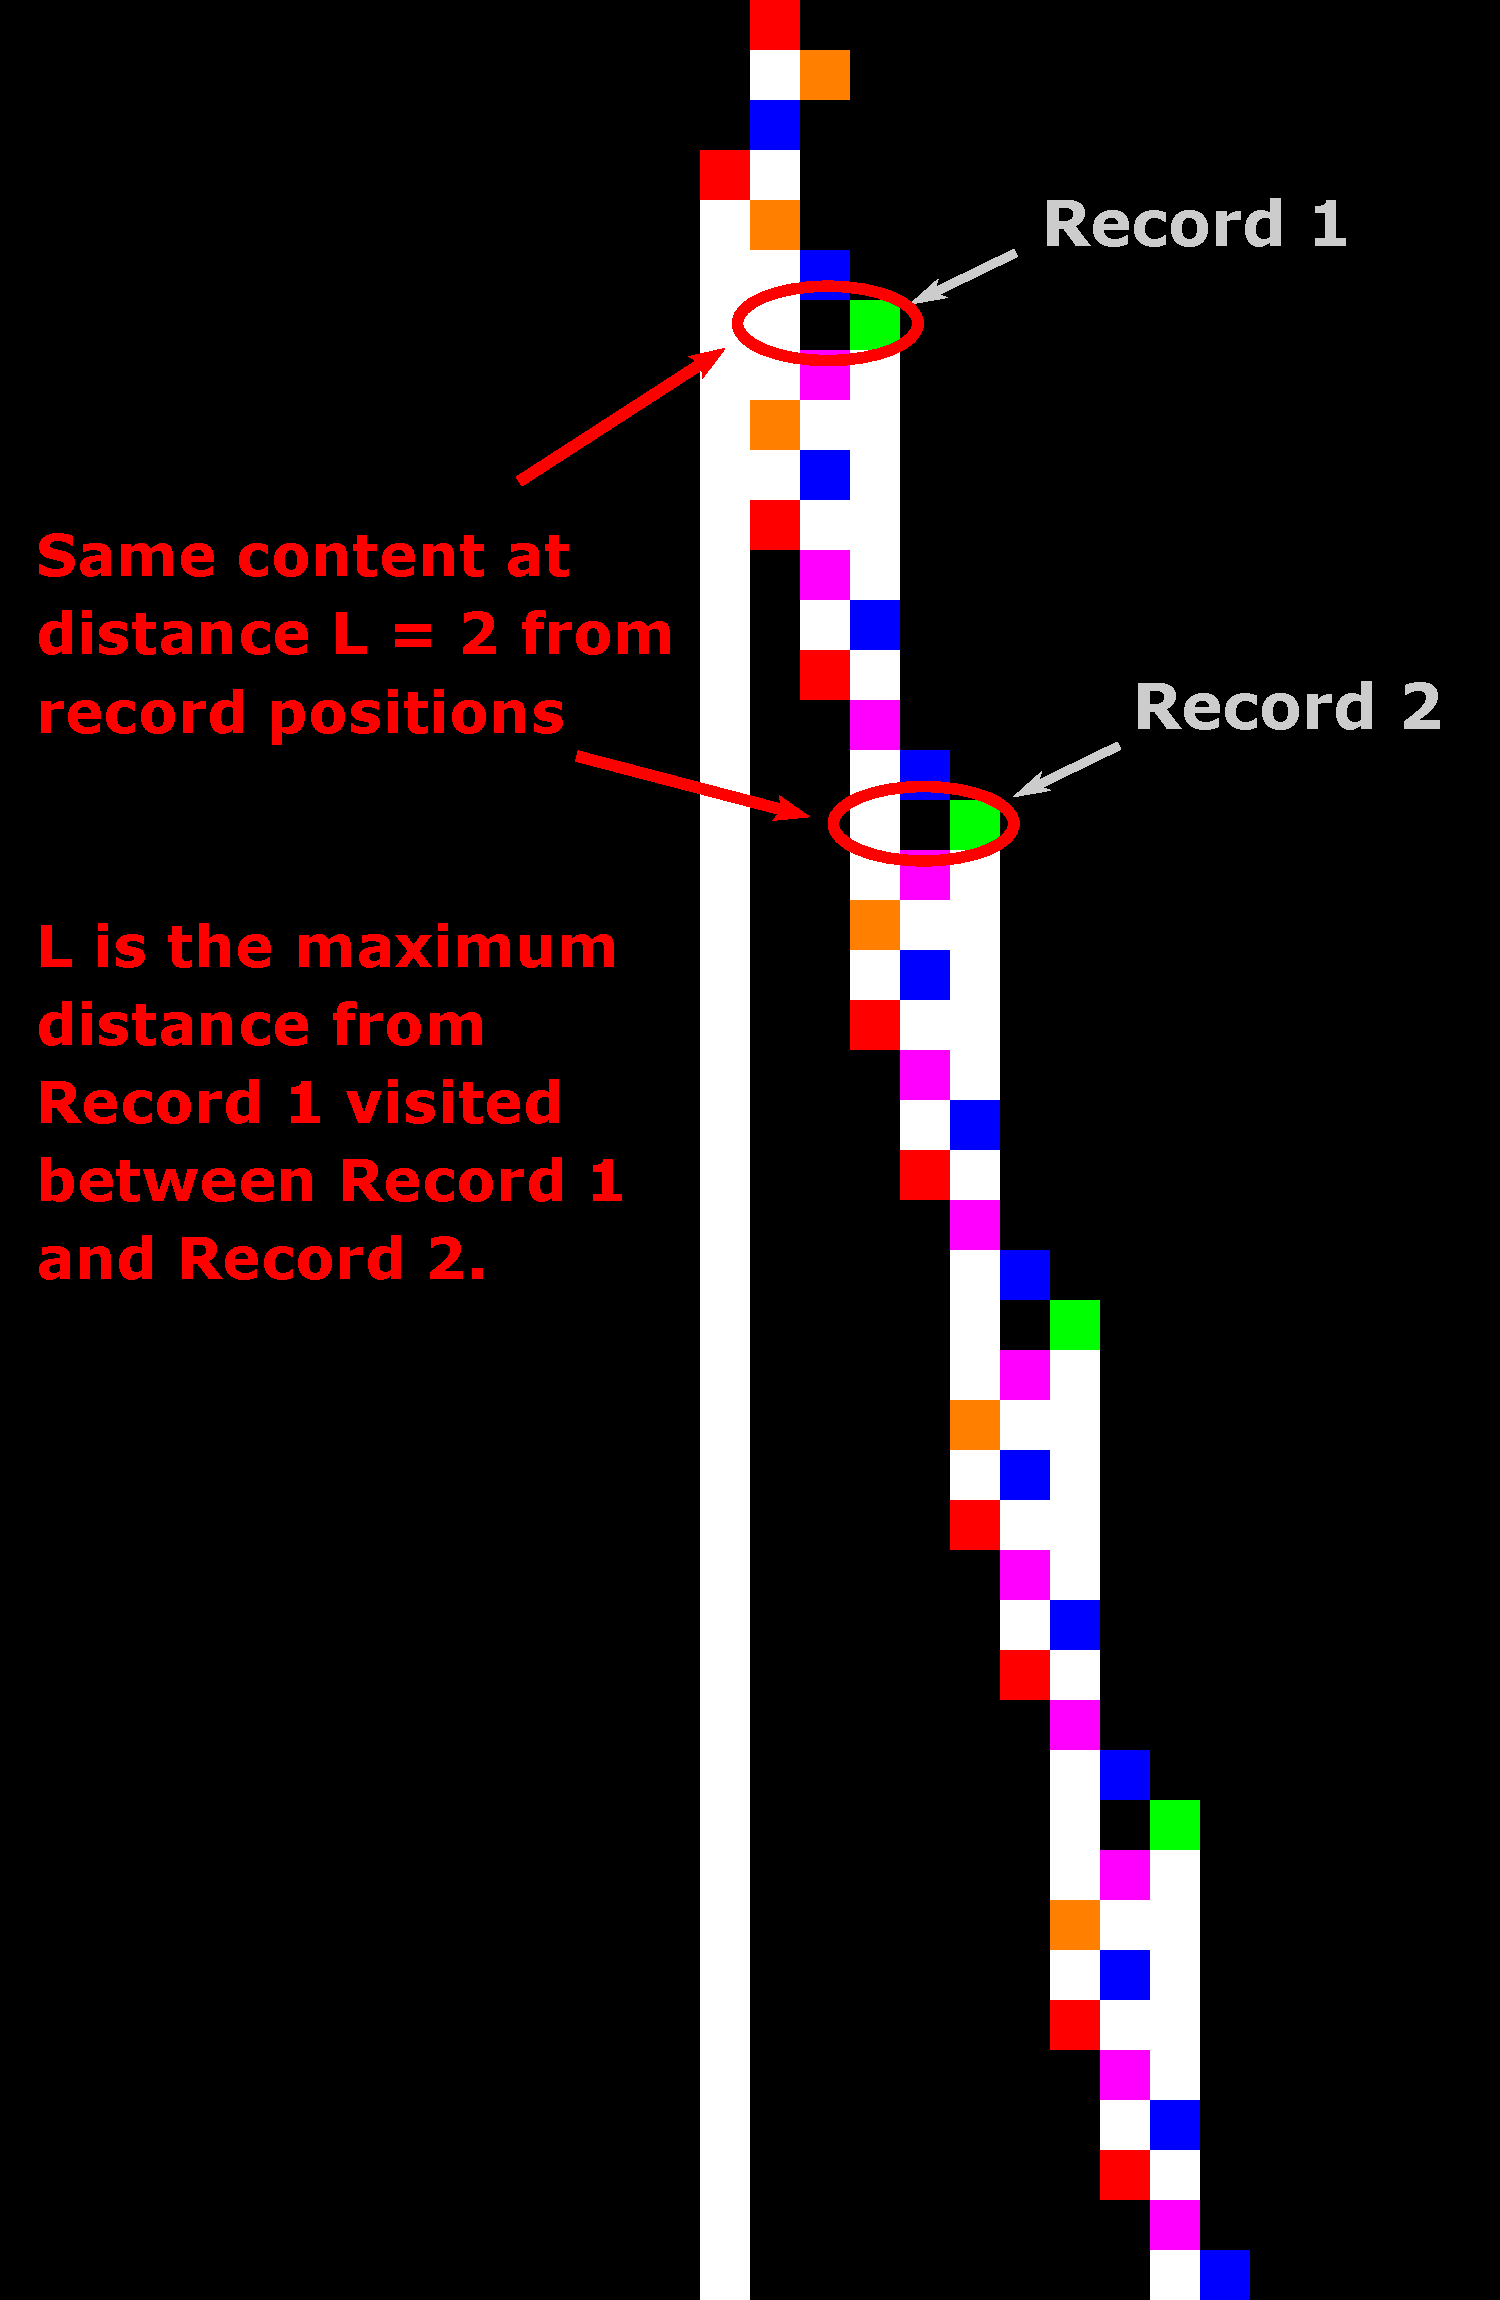
\includegraphics[width=0.54\textwidth]{space-time-diagrams/translated_cycler_44394115_annotated.pdf}

  \caption{Example ``Translated cycler'': 45-step space-time diagram of bbchallenge's machine \#44,394,115. See \url{https://bbchallenge.org/44394115}. The same bounded pattern is being translated to the right for ever. The text annotations illustrate the main idea for recognising ``Translated Cyclers'': find two configurations that break a record (i.e. visit a memory cell that was never visited before) in the same state (here state \textcolor{colorD}{D}) such that the content of the memory tape at distance L from the record positions is the same in both record configurations. Distance L is defined as being the maximum distance to record position 1 that was visited between the configuration of record 1 and record 2.}\label{fig:translated-cyclers}
  \end{figure}
  
The goal of this decider is to recognise Turing machines that translate a bounded pattern for ever. We call such machines ``Translated cyclers''. They are close to ``Cyclers'' (Section~\ref{sec:cyclers}) in the sense that they are only repeating a pattern but there is added complexity as they are able to translate the pattern in space at the same time, hence the decider for Cyclers cannot directly apply here.

The main idea for this decider is illustrated in Figure~\ref{fig:translated-cyclers} which gives the space-time diagram of a ``Translated cycler': bbchallenge's machine \#44,394,115 (c.f. \url{https://bbchallenge.org/44394115}). The idea is to find two configurations that break a record (i.e. visit a memory cell that was never visited before) in the same state (here state \textcolor{colorD}{D}) such that the content of the memory tape at distance L from the record positions is the same in both record configurations. Distance L is defined as being the maximum distance to record position 1 that was visited between the configuration of record 1 and record 2. In those conditions, we can prove that the machine will never halt.

The translated cycler of Figure~\ref{fig:translated-cyclers} features a relatively simple repeating pattern and transient pattern (pattern occurring before the repeating patterns starts). These can get significantly more complex, bbchallenge's machine \#59,090,563 is an example see Figure~\ref{fig:translated-cyclers-more} and \url{https://bbchallenge.org/59090563}. The method for detecting the behavior is the same but more resources are needed.


\begin{figure}
\centering
% 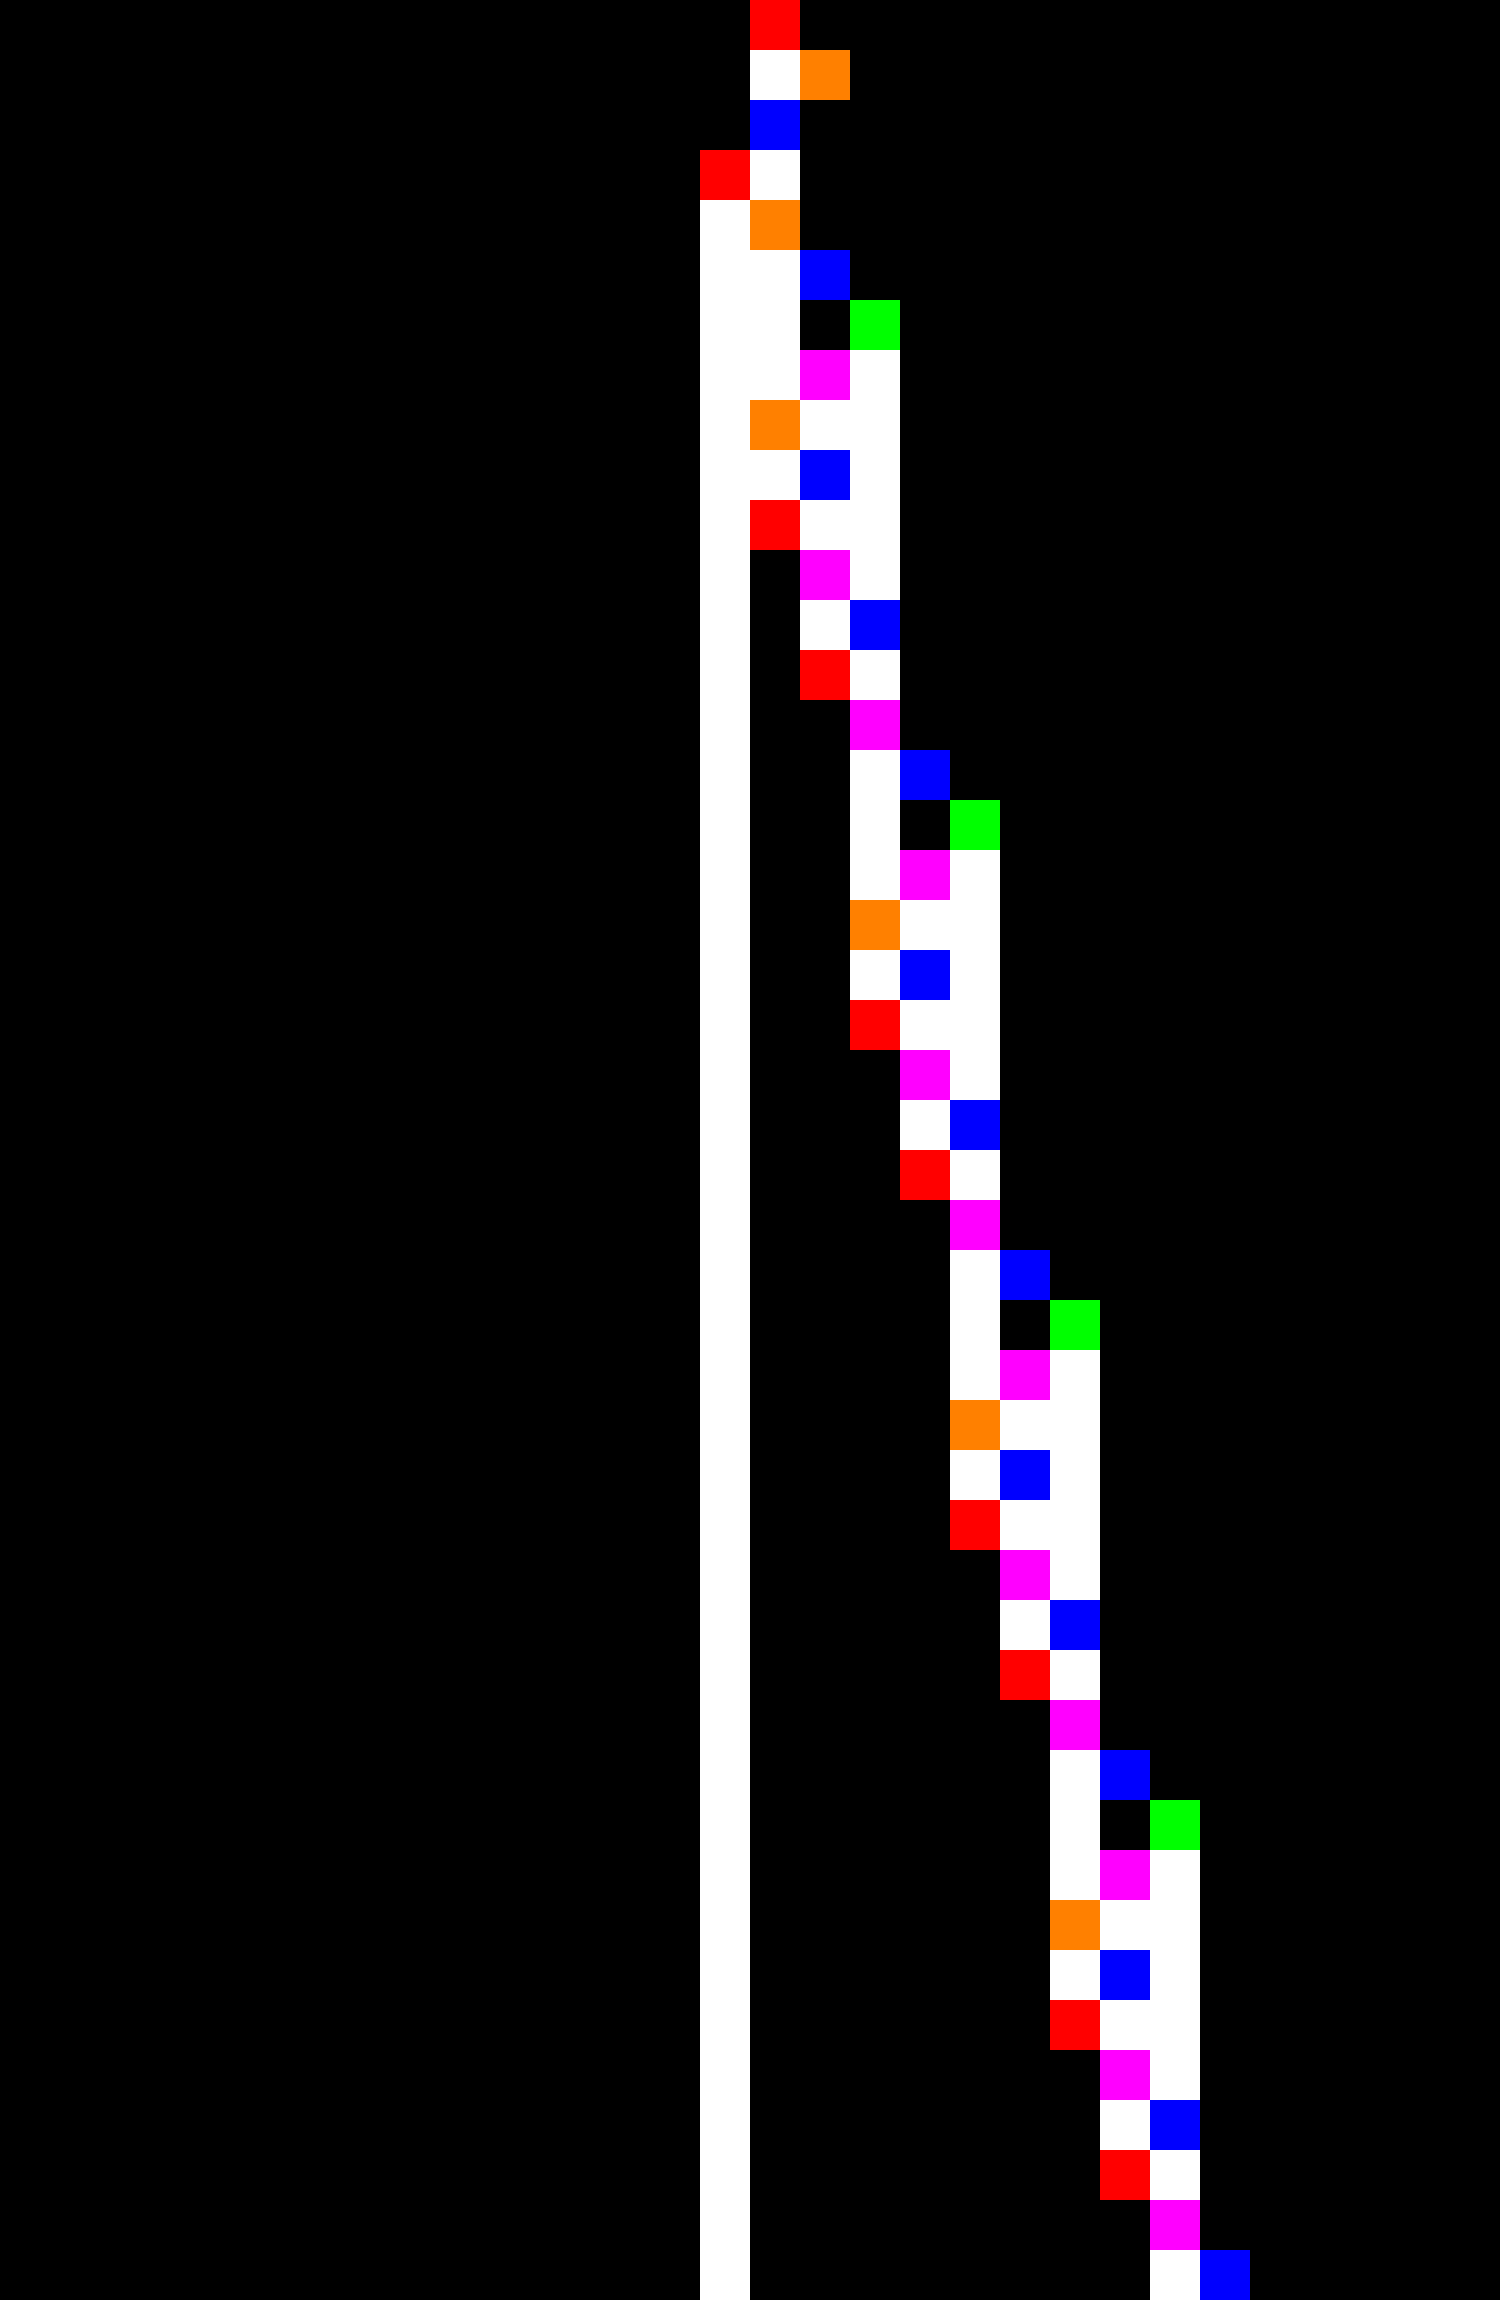
\includegraphics[width=0.5\textwidth]{space-time-diagrams/translated_cycler_44394115.pdf}
% \hspace{2ex}
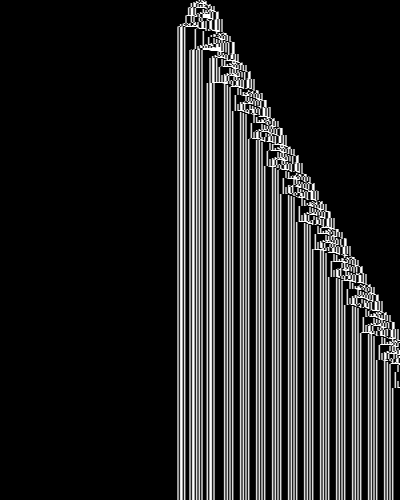
\includegraphics[width=0.7\textwidth]{space-time-diagrams/translated_cycler_59090563.png}

\caption{More complex ``Translated cycler'': 10,000-step space-time diagram (no state colours) of bbchallenge's machine \#59,090,563. See \url{https://bbchallenge.org/59090563}.}\label{fig:translated-cyclers-more}
\end{figure}


\subsection{Pseudocode}

We assume that we are given a Turing Machine type \textbf{TM} that encodes the transition table of a machine as well as a procedure \textbf{TuringMachineStep}(machine,configuration) which computes the next configuration of a Turing machine from the given configuration or \textbf{nil} if the machine halts at that step.

One minor complication of the technique described above is that one has to track record-breaking configurations on both sides of the tape: a configuration can break a record on the right or on the left. Also, in order to compute distance $L$ (see above or Definition~\ref{def:distL}) it is useful to add to memory cells the information of the last time step at which it was visited.

We also assume that we are given a routine {\sc get-extreme-position}(tape,sideOfTape) which gives us the rightmost or leftmost position of the given tape (well defined as we always manipulate finite tapes).

\begin{algorithm}
        \caption{{\sc decider-translated-cylers}}\label{alg:translated-cyclers}

        \begin{algorithmic}[1]
          \State \textbf{const int} RIGHT, LEFT = 0, 1 
          \State \textbf{struct} ValueAndLastTimeVisited \{
            \State \tabi\textbf{int} value
            \State \tabi\textbf{int} lastTimeVisited
            

            \State \}
                \State \textbf{struct} Configuration \{
                \State \tabi\textbf{int} state
                \State \tabi\textbf{int} headPosition
                \State \tabi\textbf{int $\boldsymbol{\to}$ ValueAndLastTimeVisited} tape
                \State \}
                \State 
                

                \Procedure{\textbf{bool} {\sc decider-translated-cylers}}{\textbf{TM} machine,\textbf{int} timeLimit}
                \State \textbf{Configuration} currConfiguration = \{.state = 0,$\,$.headPosition = 0,$\,$ .tape = \{0:\{.value = 0, .lastTimeVisited = 0\}\}\}
                \State // 0: right records, 1: left records
                \State \textbf{List$\boldsymbol{<}$Configuration$\boldsymbol{>}$} 
                recordBreakingConfigurations[2] = [[],[]] 
                \State \textbf{int} extremePositions[2] = [0,0]
                \State \textbf{int} currTime = 0

                \While{currTime $<$ timeLimit}
                \State \textbf{int} headPosition = currConfiguration.headPosition
                \State currConfiguration.tape[headPosition].lastTimeVisited = currTime
                \If{headPosition $>$ extremePositions[RIGHT] \textbf{or} headPosition $<$ extremePositions[LEFT]}
                \State \textbf{int} recordSide = (headPosition $>$ extremePositions[RIGHT]) ? RIGHT : LEFT
                \State extremePositions[recordSide] = headPosition
                \If{{\sc check-records}(currConfiguration, recordBreakingConfigurations[recordSide], recordSide)}
                \State \textbf{return} true
                \EndIf
                \State recordBreakingConfigurations[recordSide].\textbf{append}(currConfiguration)
                \EndIf

                \State currConfiguration = \textbf{TuringMachineStep}(machine,currConfiguration)
                \State currTime += 1


                \If{currConfiguration == \textbf{nil}}
                \State \textbf{return} false //machine has halted, it is not a Translated Cycler
                \EndIf
                \EndWhile

                \State \textbf{return} false
                \EndProcedure

        \end{algorithmic}
      \end{algorithm}
        \begin{algorithm}
        \begin{algorithmic}[1]
          \caption{{\sc compute-distance-L} and {\sc aux-check-records}}\label{alg:translated-cyclers-aux}

          \Procedure{\textbf{int} {\sc compute-distance-L}}{\textbf{Configuration} currRecord, \textbf{Configuration} olderRecord, \textbf{int} recordSide}
          \State \textbf{int} olderRecordPos = olderRecord.headPosition
          \State \textbf{int} olderRecordTime = olderRecord.tape[olderRecordPos].lastTimeVisited
          \State \textbf{int} currRecordTime = currRecord.tape[currRecord.headPosition].lastTimeVisited
          \State \textbf{int} distanceL = 0
          \For{\textbf{int} pos \textbf{in} currRecord.tape}
          \If{pos $>$ olderRecordPos \textbf{and} recordSide == RIGHT}
          \textbf{continue}
          \EndIf
          \If{pos $<$ olderRecordPos \textbf{and} recordSide == LEFT}
          \textbf{continue}
          \EndIf

          \textbf{int} lastTimeVisited = currRecord.tape[pos].lastTimeVisited
          \If{lastTimeVisited $\geq$ olderRecordTime \textbf{and} lastTimeVisited $\leq$ currRecordTime}
          \State distanceL = \textbf{max}(distanceL,\textbf{abs}(pos-olderRecordPos))
          \EndIf

          \EndFor
          \State \textbf{return} distanceL
          \EndProcedure
          \State
          \Procedure{\textbf{bool} {\sc aux-check-records} }{\textbf{Configuration} currRecord, \textbf{List$\boldsymbol{<}$Configuration$\boldsymbol{>}$} olderRecords, \textbf{int} recordSide}

                \For{\textbf{Configuration} olderRecord \textbf{in} olderRecords}
                \If{currRecord.state != olderRecord.state}
                \State \textbf{continue}
                \EndIf
                \State \textbf{int} distanceL = {\sc compute-distance-L}(currRecord,olderRecord,recordSide)
                \State \textbf{int} currExtremePos = {\sc get-extreme-position}(currRecord.tape,recordSide)
                \State \textbf{int} olderExtremePos = {\sc get-extreme-position}(olderRecord.tape,recordSide)
                \State \textbf{int} step = (recordSide == RIGHT) ? -1 : 1
                \State \textbf{bool} isSameLocalTape = true
                \For{\textbf{int} offset = 0; \textbf{abs}(offset) $<$ distanceL; offset += step}
                \If{currRecord.tape[currExtremePos+offset] != olderRecord.tape[olderExtremePos+offset]}
                \State isSameLocalTape = false
                \State \textbf{break}
                \EndIf
                \EndFor
                \If{isSameLocalTape}
                \State \textbf{return} true
                \EndIf
                \EndFor
                \State \textbf{return} false
                \EndProcedure
    
        \end{algorithmic}
\end{algorithm}

\subsection{Correctness}

\begin{definition}[record-breaking configurations]\normalfont
  Let $\mathcal{M}$ be a Turing machine and $c_0$ its busy beaver initial configuration (i.e. state is 0, head position is 0 and tape is all-0).
  Let $c$ be a configuration reachable from $c_0$, i.e. $c_0 \vdash^* c$.
Then $c$ is said to be \textit{record-breaking} if the current head position had never been visited before. Records can be broken to the \textit{right} (positive head position) or to the left (negative head position).
\end{definition}

\begin{definition}[Distance $L$ between record-breaking configurations]\label{def:distL}\normalfont
  Let $\mathcal{M}$ be a Turing machine and $r_1,r_2$ be two record-breaking configurations on the same side of the tape at respective times $t_1$ and $t_2$ with $t_1 < t_2$. Let $p_1$ and $p_2$ be the tape positions of these records. Then, distance $L$ between $r_1$ and $r_2$ is defined as $\max\{|p_1 - p|\}$ with $p$ any position visited by $\mathcal{M}$ between $t_1$ and $t_2$ that is not beating record $p_1$ (i.e. $p \leq p_1$ for a record on the right and $p \geq p_1$ for a record on the left). 
\end{definition}

\begin{lemma}\label{lem:translated-cyclers}\normalfont 
Let $\mathcal{M}$ be a Turing machine. Let $r_1$ and $r_2$ be two configurations that broke a record in the same state and on the same side of the tape at respective times $t_1$ and $t_2$ with $t_1 < t_2$. Let $p_1$ and $p_2$ be the tape positions of these records. Let $L$ be the distance between $r_1$ and $r_2$ (Definition~\ref{def:distL}). If the content of tape in $r_1$ at distance $L$ of $p_1$ is the same than the content of the tape in $r_2$ at distance $L$ of $p_2$ then $\mathcal{M}$ never halts. Furthermore, by Definition~\ref{def:distL}, we know that distance $L$ is the maximum distance that $\mathcal{M}$ can travel to the left of $p_1$ between times $t_1$ and $t_2$.
\end{lemma}

\begin{proof}\normalfont
Let's suppose that the record-breaking configurations are on the right-hand side of the tape. By the hypotheses, we know the machine is in the same state in $r_1$ and $r_2$ and that the content of the tape at distance $L$ to the left of $p_1$ in $r_1$ is the same as the content of the tape at distance $L$ to the left of $p_2$ in $r_2$. Note that the content of the tape to the right of $p_1$ and $p_2$ is the same: all-0 since they are record positions. Hence that after $r_2$, since it will read the same tape content the machine will reproduce the same behavior than it did after $r_1$ but translated at position $p_2$: there will a record-breaking configuration $r_3$ such that the distance between record-breaking configurations $r_2$ and $r_3$ is also $L$ (Definition~\ref{def:distL}). Hence the machine will keep breaking records to the right for ever and will not halt. Analogous proof for records that are broken to the left.
\end{proof}

\begin{theorem}\label{th:translated-cyclers}\normalfont
  Let $\mathcal{M}$ be a Turing machine and $t$ a time limit. The conditions of Lemma~\ref{lem:translated-cyclers} are met before time $t$ if and only if {\sc decider-translated-cyclers}($\mathcal{M}$,$t$) outputs \texttt{true} (Algorithm~\ref{alg:translated-cyclers}).
\end{theorem}
\begin{proof}
The algorithm consists of a main function {\sc decider-translated-cyclers} (Algorithm~\ref{alg:translated-cyclers}) and two auxiliary functions {\sc compute-distance-L} and {\sc aux-check-records} (Algorithm~\ref{alg:translated-cyclers-aux}).

The main loop of {\sc decider-translated-cyclers} (Algorithm~\ref{alg:translated-cyclers} l.17) simulates the machine with the particularity that (a) it keeps track of the last time it visited each memory cell (l.19) and (b) it keeps track of all record-breaking configurations that are met (l.20) before reaching time limit $t$. When a record-breaking configuration is found, it is compared to all the previous record-breaking configurations on the same side in seek of the conditions of Lemma~\ref{lem:translated-cyclers}. This is done by auxiliary routine {\sc aux-check-records} (Algorithm~\ref{alg:translated-cyclers-aux}).

Auxiliary routine {\sc aux-check-records} (Algorithm~\ref{alg:translated-cyclers-aux}, l.12) loops over all older record-breaking configurations on the same side than the current one (l.13). The routine ignores older record-breaking configurations that were not in the same state than the current one (l.14). If the states are the same, it computes distance $L$ (Definition~\ref{def:distL}) between the older and the current record-breaking configuration (l.16). This computation is done by auxiliary routine {\sc compute-distance-L}.

Auxiliary routine {\sc compute-distance-L} (Algorithm~\ref{alg:translated-cyclers-aux}, l.1) uses the ``pebbles'' that were left on the tape to give the last time a memory cell was seen (field \texttt{lastTimeVisited}) in order to compute the farthest position from the old record position that was visited before meeting the new record position (l.10). Note that we discard intermediate positions that beat the old record position (l.7-8) as we know that the part of the tape after the record position in the old record-breaking configuration is all-0, same as the part of the tape after current record position in the current record-breaking position (part of the tape to the right of the red-circled green cell in Figure~\ref{fig:translated-cyclers}).

Thanks to the computation of {\sc compute-distance-L} the routine {\sc aux-check-records} is able to check whether the tape content at distance $L$ of the record-breaking position in both record-holding configurations is the same or not (Algorithm~\ref{alg:translated-cyclers-aux}, l.22). The routine returns \texttt{true} if they are the same and the function {\sc decider-translated-cyclers} will return \texttt{true} as well in cascade (Algorithm~\ref{alg:translated-cyclers} l.24). That scenario is reached if and only if the algorithm has found two record-breaking configurations on the same side that satisfy the conditions of Lemma~\ref{lem:translated-cyclers}, which is what we wanted.

\end{proof}

\begin{corollary}\normalfont
  Let $\mathcal{M}$ be a Turing machine and $t \in \mathbb{N}$ a time limit. If {\sc decider-translated-cyclers}($\mathcal{M}$,$t$) returns \texttt{true} then the behavior of $\mathcal{M}$ from all-0 tape has been decided: $\mathcal{M}$ does not halt.
\end{corollary}
\begin{proof}
Immediate by combining Lemma~\ref{lem:translated-cyclers} and Theorem~\ref{th:translated-cyclers}.
\end{proof}

\subsection{Results}

The decider was coded in \texttt{golang} and is accessible at this link: \url{https://github.com/bbchallenge/bbchallenge-deciders/tree/main/decider-translated-cyclers}.

The decider found 73,860,604 ``Translated cyclers'', out of 88,664,064 machines in the seed database of the Busy Beaver Challenge (c.f. \url{https://bbchallenge.org/method#seed-database}). More information about these results are available at: \url{https://discuss.bbchallenge.org/t/decider-translated-cyclers/34}.
\section{Decider for backward reasoning}\label{sec:backward-reasoning}

\begin{figure}
  \centering
  \begin{subfigure}[m]{0.45\textwidth}
      \centering
      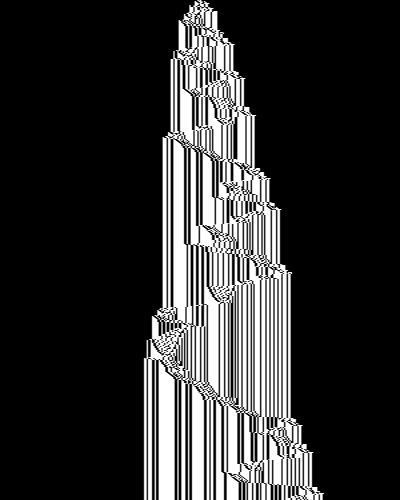
\includegraphics[width=\textwidth]{space-time-diagrams/backward_reasoning_55897188.png}
      \caption{10,000-step space-time diagram of bbchalenge's machine \#55,897,188. \url{https://bbchallenge.org/55897188}}
      \label{fig:y equals x}
  \end{subfigure}
  \hfill
  \begin{subfigure}[m]{0.45\textwidth}
      \centering
      \begin{tabular}{lll}
        & 0   & 1   \\
      \textcolor{colorA}{A} & 1R\textcolor{colorB}{B} & 0LD \\
      \textcolor{colorB}{B} & 1L\textcolor{colorC}{C} & 0RE \\
      \textcolor{colorC}{C} & - - - & 1LD \\
      D & 1LA & 1LD \\
      E & 1RA & 0RA
      \end{tabular}
      
      
      \caption{Transition table of machine \#55,897,188.}
      
  \end{subfigure}
  
  \begin{subfigure}[m]{1\textwidth}
    \vspace{5ex}
    \centering
    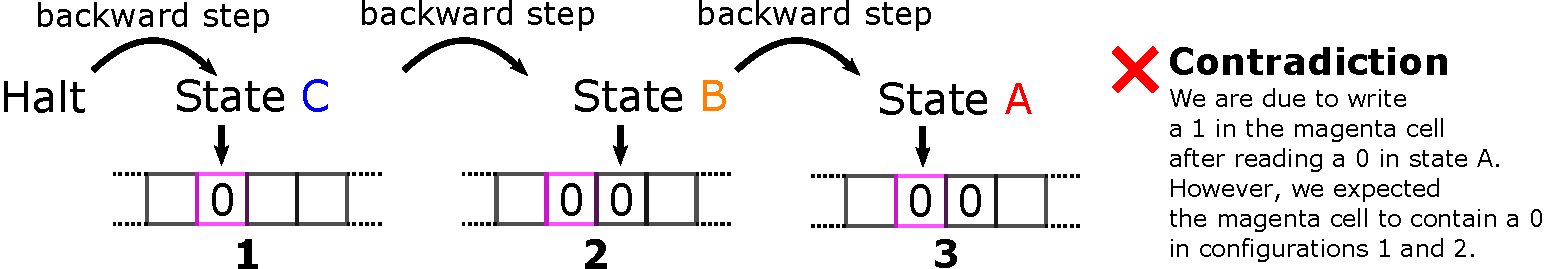
\includegraphics[width=0.9\textwidth]{backward-reasoning.pdf}
    
    \caption{Contradiction reached after 3 backward steps: machine \#55,897,188 does cannot reach its halting configuration hence it does not halt.}
    
\end{subfigure}
  
     \caption{Applying backward reasoning on bbchallenge's machine \#55,897,188. (a) 10,000-step space-time diagram of machine \#55,897,188. The \textit{forward} behavior of the machine looks very complex. (b) Transition table. (c) We are able to deduce that the machine will never halt thanks to only 3 backward reasoning steps: because a contradiction is met, it is impossible to reach the halting configuration in more than 3 steps -- and, by (a), the machine can do at least 20,000 without halting.}
     \label{fig:backward-reasoning}
\end{figure}


Backward reasoning, as described in \cite{Marxen_1998}, takes a different approach than what has been done with deciders in Sections~\ref{sec:cyclers} and \ref{sec:translated-cyclers}. Indeed, instead of trying to recognise a particular kind of machine's behavior, the idea of backward reasoning is to show that, independently of the machine's behavior, the halting configurations are not reachable. In order to do so, the decider simulates the machine \textit{backwards} from halting configurations until it reaches some obvious contradiction. 

Figure~\ref{fig:backward-reasoning} illustrates this idea on bbchallenge's machine \#55,897,188. From the space-time diagram, the \textit{forward} behavior of the machine from all-0 tape looks to be extremely complex, Figure~\ref{fig:backward-reasoning}a. However, by reconstructing the sequence of transitions that would lead to the halting configuration (reading a 0 in state \textcolor{colorC}{C}), we reach a contradiction in only 3 steps, Figure~\ref{fig:backward-reasoning}c. Indeed, the only way to reach state  \textcolor{colorC}{C} is to come from the right in state \textcolor{colorB}{B} where we read a 0. The only way to reach state \textcolor{colorB}{B} is to com from left in state  \textcolor{colorA}{A} where we read a 0. However, the transition table (Figure~\ref{fig:backward-reasoning}b) is instructing us to write a 1 in that case, which is not consistent with the 0 that we assumed was at position in order for the machine to halt.

Backward reasoning in the case of Figure~\ref{fig:backward-reasoning} was particularly simple because there was only one possible previous configuration for each backward step -- e.g. there is only one transition that can reach state \textcolor{colorC}{C} and same for state \textcolor{colorB}{B}. In general, this is not the case and the structure created by backward reasoning is a tree of configurations instead of just a chain. If all the leaves of a backward reasoning tree of depth $D$ reach a contradiction, we know that if the machine runs for $D$ steps from all-0 tape then the machine cannot reach a halting configuration and thus does not halt.

\subsection{Pseudocode}

\begin{algorithm}
  \caption{{\sc decider-backward-reasoning}}\label{alg:backward-reasoning}

  \begin{algorithmic}[1]
    \State{\textbf{const int} RIGHT, LEFT = 0, 1}
    \State \textbf{struct} Transition \{
      \State \tabi\textbf{int} state, read, write, move
      \State \}
          \State \textbf{struct} Configuration \{
          \State \tabi\textbf{int} state
          \State \tabi\textbf{int} headPosition
          \State \tabi\textbf{int $\boldsymbol{\to}$ int} tape
          \State \tabi\textbf{int} depth
          \State \}
         
          \State
          
          \Procedure{\textbf{Configuration} {\sc apply-transition-backwards}}{\textbf{Configuration} conf,\textbf{Transition} t}
          \State \textbf{int} reversedHeadMoveOffset = (t.move == RIGHT) ? -1 : 1
          \State \textbf{int} previousPosition = conf.headPosition+reversedHeadMoveOffset
          \State // Backward contradiction spotted
          \If{previousPosition \textbf{in} conf.tape \textbf{and} conf.tape[previousPosition] != t.write}
          \State \textbf{return} \textbf{nil}
          \EndIf
          \State \textbf{Configuration} previousConf = \{.state = t.state, .depth = conf.depth + 1, .tape = conf.tape\}
          \State previousConf.headPosition = previousPosition
          \State previousConf.tape[previousPosition] = t.read
          \State \textbf{return} previousConf
          \EndProcedure
          \State
          \Procedure{\textbf{bool} {\sc decider-backward-reasoning}}{\textbf{TM} machine,\textbf{int} maxDepth}
          
          \State \textbf{Stack$\boldsymbol{<}$Configuration$\boldsymbol{>}$} configurationStack
          \For{\textbf{int} (state,read) \textbf{in} {\sc get-undefined-transitions}(machine)}
          \State \textbf{Configuration} haltingConfiguration = \{.state = state,.depth=0,.headPosition = 0\}
          \State haltingConfiguration.tape = \{0: read\}
          \State configurationStack.\textbf{push}(haltingConfiguration)
          \EndFor
          \State \textbf{Set$\boldsymbol{<}$Configuration$\boldsymbol{>}$} configurationsSeen = \{\}
          \While{!configurationStack.\textbf{empty}() \textbf{ and }configurationStack.\textbf{top}().depth $<$ maxDepth}
          \State \textbf{Configuration} currConf = configurationStack.\textbf{pop}()
          \If{currConf \textbf{in} configurationsSeen} \textbf{continue} \EndIf
          \State configurationsSeen.\textbf{insert}(currConf)
          \State \textbf{List$\boldsymbol{<}$Configuration$\boldsymbol{>}$} confList = []
          
          \For{\textbf{Transition} transition \textbf{in} {\sc get-transitions-reaching-state}(machine,currConf.state)}
          \State \textbf{Configuration} previousConf = {\sc apply-transition-backwards}(currConf, transition)
          \State // If no contradiction
          \If{previousConf != \textbf{nil}}
          \State configurationStack.\textbf{push}(previousConf)
          \EndIf
          \EndFor
          \EndWhile

          \State // Returns true iff all leaves at depth $\leq$ maxDepth reached a contradiction
          \State \textbf{return} configurationStack.\textbf{empty}()
          \EndProcedure

  \end{algorithmic}
\end{algorithm}

We assume that we are given routine {\sc get-undefined-transitions}(machine) which returns the list of (state,readSymbol) pairs of all the undefined transitions in the machine's transition table, for instance [(\textcolor{colorC}{C},0)] for the machine of Figure~\ref{fig:backward-reasoning}b. We also assume that we are given routine {\sc get-transitions-reaching-state}(machine,targetState) which returns the list of all machine's transitions that go to the specified target state, for instance [(\textcolor{colorA}{A},1,0LD),(\textcolor{colorC}{C},1,1LD),(D,1,1LD)] for target state D in the machine of Figure~\ref{fig:backward-reasoning}b. These two routines contain very minimal logic as they only lookup in the description of the machine for the required information.

\subsection{Correctness}

\begin{theorem}\label{th:backward-reasoning}\normalfont
  Let $\mathcal{M}$ be a Turing machine and $D\in\mathbb{N}$.
  Then, {\sc decider-backward-reasoning}($\mathcal{M}$,$D$) returns \texttt{true} if and only if no undefined transition of $\mathcal{M}$ can be reached in more than $D$ steps.
\end{theorem}
\begin{proof}
The tree of backward configurations is maintained in a DFS fashion through a stack (Algorithm~\ref{alg:backward-reasoning}, l.24). Initially, the stack is filled with the configurations where only one tape cell is defined and state is set such that the corresponding transition is undefined (i.e. the machine halts after that step), l.25-28. 

Then, the main loop runs until either (a) the stack is empty or (b) maximum depth has been reached, l.30. Note that running the algorithm with increased maximum depth increases its chances to contradict all branches of the backward simulation tree. At each step of loop, we remove the current configuration from the stack and we try to apply all the transitions that leads to its state backwards by calling routine {\sc apply-transition-backwards}(configuration, transition).

The only case where it is not possible to apply a transition backwards, i.e. the case where a contradiction is reached is when the tape symbol at the position where the transition comes from (i.e. to the right if transition movement is left and vice-versa) is defined but is not equal to the write instruction of the transition. Indeed, that means that the future (i.e. previous backward steps) is not consistent the current transition's write instruction. This logic is checked l.16. Otherwise, we can construct the previous configuration (i.e. next backward step) and augment depth by 1. We then stack this configuration in the main routine (l.39).

The algorithm returns \texttt{true} if and only if the stack ever becomes empty which means that all leaves of the backward simulation tree of depth $D$ have reached a contradiction and thus, no undefined transition of the machine is reachable in more than $D$ steps.

This pseudocode contains a slight optimisation with the use of set \texttt{configurationSeen} (l.29). This set racks configurations which would have already been seen in different branches of the tree in order not traverse them twice (l.32-33). While not needed in theory, this optimisation is useful in practice, especially at large depths (e.g. $D=300$).
\end{proof}

\begin{corollary}\normalfont
  Let $\mathcal{M}$ be a Turing machine and $D\in\mathbb{N}$. If {\sc decider-backward-reasoning}($\mathcal{M}$,$D$) returns \texttt{true} and machine $\mathcal{M}$ can run $D$ steps from all-0 tape without halting then the behavior of $\mathcal{M}$ from all-0 tape has been decided: $\mathcal{M}$ does not halt.
\end{corollary}
\begin{proof}
By Theorem~\ref{th:backward-reasoning} we know that no undefined transition of $\mathcal{M}$ can be reached in more than $D$ steps. Hence, if machine $\mathcal{M}$ can run $D$ steps from all-0 tape without halting, it will be able to run the next $D+1^{\text{th}}$ step. From there, the machine cannot halt or it would contradict the fact that halting trajectories have at most $D$ steps. Hence, $\mathcal{M}$ does not halt from all-0 tape.
\end{proof}



\bibliographystyle{abbrv}
\bibliography{correctness-deciders}

\end{document}